\section{Background and Related Works}
\label{sec:background}
In this section, we review some issues related to developing an event-based middleware for WSN. We also briefly discuss the works that have done so far to address those issues
We first briefly overview the basic concepts r These concepts will be used extensively when we describe our design for PSWare.

\subsection{WSN-based Middleware}
WSN brings a lot of opportunities as well as some challenges. WSN allows large scale deployment and have a large area of applications. However, developing WSN-based applications is considered challenging because of the following issues.

\emph{Abstraction Support}: WSN usually consists of large number of heterogeneous sensors. These sensors may be developed by different vendors and may have different capability, precision and platform. Therefore, the middleware should hide the underlying platform details and provide a high level programming paradigm for the application programmers. Ideally, a good programming paradigm allows programming the sensor network as a single 'virtual' entity, rather than individual nodes \cite{programmingparadigms}.

\emph{Resource Constraints}: usually each sensor node in the network has limited resources like energy, computing power, memory and communication bandwidth. Hence, middleware components have to be lightweight to fit these constraints. Middleware should also provide support to dynamically adapt performance and resource consumption to the varying needs of the application, for example, by enabling dynamic tradeoffs between output quality and resource consumption. In addition, multiple applications may run on the same network so the middleware need to fairly allocate resources between different applications.

Consequently, a lot of middleware works have been proposed to help on these issues. Existing works on middleware may be categorized according to the programming abstractions they provide including query-based approach, virtual machine-based approach and agent-based approach. Query-based approach views the whole network as a database. The data collected by the sensor nodes are ordered to facilitate the query operations. A representative work in this category is TinyDB \cite{tinydb}.

Agent is another popular programming abstraction for WSN applications. One of the motivations to use agent-based approach is to allow multiple applications to be executed on the same network. Therefore, the codes running on individual sensor nodes are treated as mobile agents and may move between different sensor nodes. A representative work is Agilla \cite{agilla}.

Apart from query and agent, virtual machine is another approach for programming abstraction. In this approach, the middleware provides instruction sets to the upper layer applications. Each instruction is usually linked with an underlying function or handler provided in the middleware. The benefit for such approach is that it is possible to have higher level abstractions on top of the instruction set. For example, a query-based scripting language may be built on top of a VM if the underlying instructions can support query operations effectively. A representative work from this category is Mat\'{e} \cite{mate}.

As discussed in Section \ref{sec:introduction}, many WSN applications are event-based. This may make the query based approach unsuitable for some of the applications since SQL or agent may not be able to express the temporal and spatial relations among different events. In this paper, we propose an event-based middleware named PSWare. Different from the existing event-based middleware, PSWare can support composite events. In addition, PSWare uses a flexible architecture. On the top level, PSWare provides an event definition language which can be used to define composite events. On the lower level, PSWare uses an architecture similar to a virtual machine where different event processing algorithms can be easily integrated by implementing different byte codes.

\subsection{Primitive Events and Filters}
Before describing the design of our middleware, we first overview the event model incorporated by PSWare. In our event model, each event is a list of attributes which are the actual data obtained from the sensor networks. For instance, the temperature and humidity readings in a room can be treated as an event. Events can be primitive or composite. In our event model, primitive events are those that can be directly sensed and obtained by individual sensor nodes.

In practical applications, the user may be only interested in a subset of the events detected by the system. This can be done through event filters (or event subscriptions from the user's point of view). Event filters are constraints applied to individual events. For instance, 'temperature \textgreater 30' may be considered as a filter. Depending on the underlying model, there are mainly three types of subscriptions: content-based, topic-based and type-based \cite{facespubsub}. Continuing with our example, 'temperature \textgreater 30' is content-based filter. If the user is interested in all the humidity readings, then a topic-based subscription can be made which so that the user only subscribes to the humidity readings. 

Compared with topic-based and content-based subscription, type-based subscription is more fine-grained. In this type of subscription, the user first specify the event types. This is similar to defining new types in many programming languages. Since each event is defined as a list of attributes, an event type defines the data types of attributes. For example, we can specify a new event type for fire alarm consisting of both humidity and temperature readings. Apart from attribute definition, the event types can also include operators for each attribute. Continuing with our example, we can define the condition for the fire alarm when the temperature reaches a certain threshold while the humidity is below another. 

There are a few works for primitive event processing in WSN. Low-level naming \cite{lowlevelnaming} is a pub/sub system based on Directed Diffusion \cite{directeddiffusion}. Attribute-based communication is used. Matching rules based on actual and formal can be defined. Filters are defined as the software modules that will be executed once triggered by matching rules. Based on these ideas the authors implement a pub/sub system for sensor network where sensor nodes can subscribe to interesting attributes. Diffusion filters \cite{diffusionfilters} extended low-level naming with a more detailed discussion on filters. The gradient filter is used to send reinforcement of transmission paths. The filters can also be used to implement GEAR (Geographic and Energy-Aware Routing) which is a geographic routing protocol.

Mires \cite{mires} is a pub/sub middleware leveraging the message-oriented communication scheme provided by the underlying TinyOS. Initially, each sensor node advertises their sensor through a multi-hop routing protocol. Then based on the advertisements, the users can make subscriptions. The subscriptions are flooded in the network using another flooding protocol. After that, the subscribed data are transmitted back to the sink with the multi-hop routing protocol.

Other works may only emphasize on a special issue in developing such event-based system. For example, \cite{sp} discusses the trade-off between reliability and energy consumption. Instead of propagating the subscription into the whole network, the authors choose to stop forwarding the subscription after a certain number of hops. The publisher will then deliver the events in an opportunistic way. If a node with subscription information is reached, the events will be delivered. Otherwise, the events will be forwarded with a certain probability.

\subsection{Composite Events}
In PSWare, we use type-based subscription because composite events can be more easily defined by specifying their types and the corresponding filters. This is similar to many programming languages where composite data types can be defined based on primitive types. Since primitive events can be directly obtained by individual sensor nodes, each composite event will usually have to be collaboratively detected by more than one sensor nodes. 

In our event model, composite events are expressed with the following steps:
\begin{enumerate}
\item Define the primitive event types that will be used for the composite events. 
\item Define the composite event type and specify what sub-event types will be used.
\item Establish the relations between the sub-events through operators.
\end{enumerate}

\begin{figure}
\centering
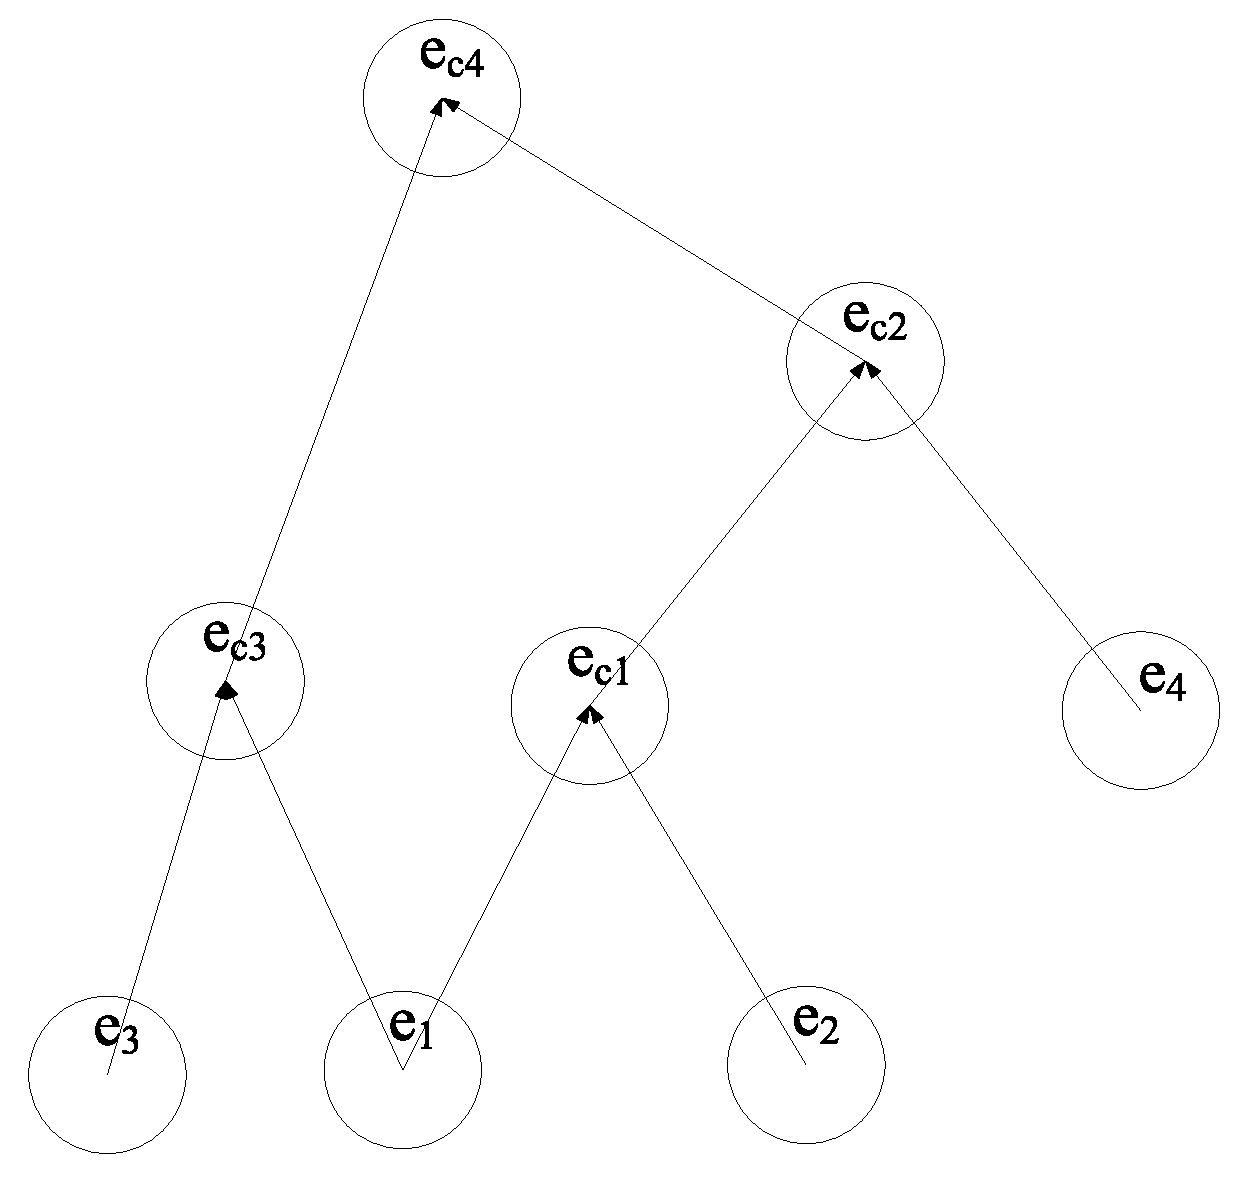
\includegraphics[width=.5\textwidth]{eventhierarchy}
\caption{Event hierarchy}
\label{fig:eventhierarchy}
\end{figure}

As we can see, in our event model, the event relations are defined through event filters. Event types together with their relations can be represented as a directed acyclic graph where each node represents an event and the each edge represents a relation. Figure \ref{fig:eventhierarchy} shows an example of such a graph. The nodes with 0 in-degree represent primitive events. The rest of the nodes represent composite events. The event which has 0 out-degree is the subscribed event.

Once the subscriptions are defined, it will be disseminated into the network so that sensor nodes can start to monitor. The sensor nodes collect data in rounds. In each round, the collected data will be matched against the subscription. If an event is found to match the subscribed event type, it will be delivered to the sink to notify the subscriber.

A few recent works such as \cite{lai:ted, complexevent} have been proposed for composite event definition and detection. The primary focus of \cite{lai:ted} is on a composite event detection algorithm called TED which utilizes event type information for efficient detection. In addition to an event language, \cite{complexevent} also discusses how to reliably detect composite events in a pervasive environment. Different from the previous works, the focus of this paper is on a flexible middleware framework so that different event detection algorithms may be integrated and evaluated easily.

\subsection{Composite Event Detection}
Composite event detection was a popular topic in the area of active database. However, for WSN, there have been very limited works. A related area is data aggregation since such work also discuss how to . Existing data aggregation can be mainly divided into three categories: cluster-based approach, \cite{leach, iheed}, chain-based approach \cite{pegasis} and tree-based approach \cite{mfst, dctc}. Cluster-based approach typically considers the problem how to select and rotate cluster heads so that the clusters can be evenly distributed in the network  and energy consumption will be balanced. A representative work is iHeed \cite{iheed}. Cluster-based approach can be organized into multiple levels in order to further save the cost.

Chain-based approach improves cluster-based approach by letting each sensor node only communicate with its close neighbors. The resulting problem is indeed very similar to traveling sales person problem. PEGASIS \cite{pegasis} is a representative work. Tree-based approaches utilize many techniques from graph theory and perform optimization. For example, \cite{xue:lp} formulates the problem as a multi-commodity flow problem and uses linear programming to solve it.  MFST \cite{mfst} constructs a minimum Steiner tree with a cost model that considers the fusion cost.

If we take the event relations into consideration while detecting the events, then detection can be done with different strategies. In this paper, we mainly consider message cost as event detection cost. Furthermore, since primitive event can be detected by individual sensor nodes, we mainly consider the composite event detection cost in this paper.

In general, if a composite event is detected based on two sub-events \(e_1\) and \(e_2\) as shown in Figure \ref{fig:event-detection2} then the cost for detecting the composite event will be the cost for detecting each individual events together with the cost for delivering the event detection results to the event detector. An event detector here is simply a node responsible for detecting composite events.

\begin{figure}
\centering
\subfloat[Basic composite event detection]{\label{fig:event-detection2}\figurehalfwidth{event-detection2}}
\subfloat[Composite event detection using event probability]{\label{fig:event-detection3}\figurehalfwidth{event-detection3}}
\caption{Composite event detection}
\label{fig:event-detection}
\end{figure}

Sometimes the events may have dependency and certain events must happen before others. In this case, we don't need to make all sensor nodes monitor the events at all the time. Instead, some nodes may firstly put to sleep mode and then be waken up when other events occur. For example, as shown in Figure \ref{fig:event-detection3}, if we have two events \(e_1\) and \(e_2\) which have a relation such that the composite event happens only when both events have been successfully detected. If \(e_2\) and \(e_1\) need to satisfy a relation such that \(e_2\) happens after \(e_1\). Then originally the nodes responsible for monitoring \(e_2\) may be put to sleep mode. After \(e_1\) has successfully been detected, a message can be forwarded to the nodes responsible for detecting \(e_2\) and wake them up. In this way, we can further reduce the energy cost because \(e_2\) doesn't have to be monitored if \(e_1\) doesn't occur.
